\chapter{Metode Penelitian}\label{ch:method}

Bab ini menguraikan tahapan penelitian yang dilakukan dalam penyusunan Tugas Akhir, meliputi studi literatur, pengumpulan dan pengolahan data, peramalan \textit{market rate}, pembentukan model optimasi berbasis MCCaR, penyelesaianmodel menggunakan metode pembanding dan \textit{Komodo Mlipir Algorithm} (KMA), analisis hasil, serta penarikan kesimpulan. Alur penelitian secara umum disajikan pada Gambar~\ref{fig:flowchart-mccar}.

\usetikzlibrary{shapes.geometric, arrows.meta, positioning, calc}

\begin{figure}[H]
\centering
\resizebox{0.78\textwidth}{!}{%
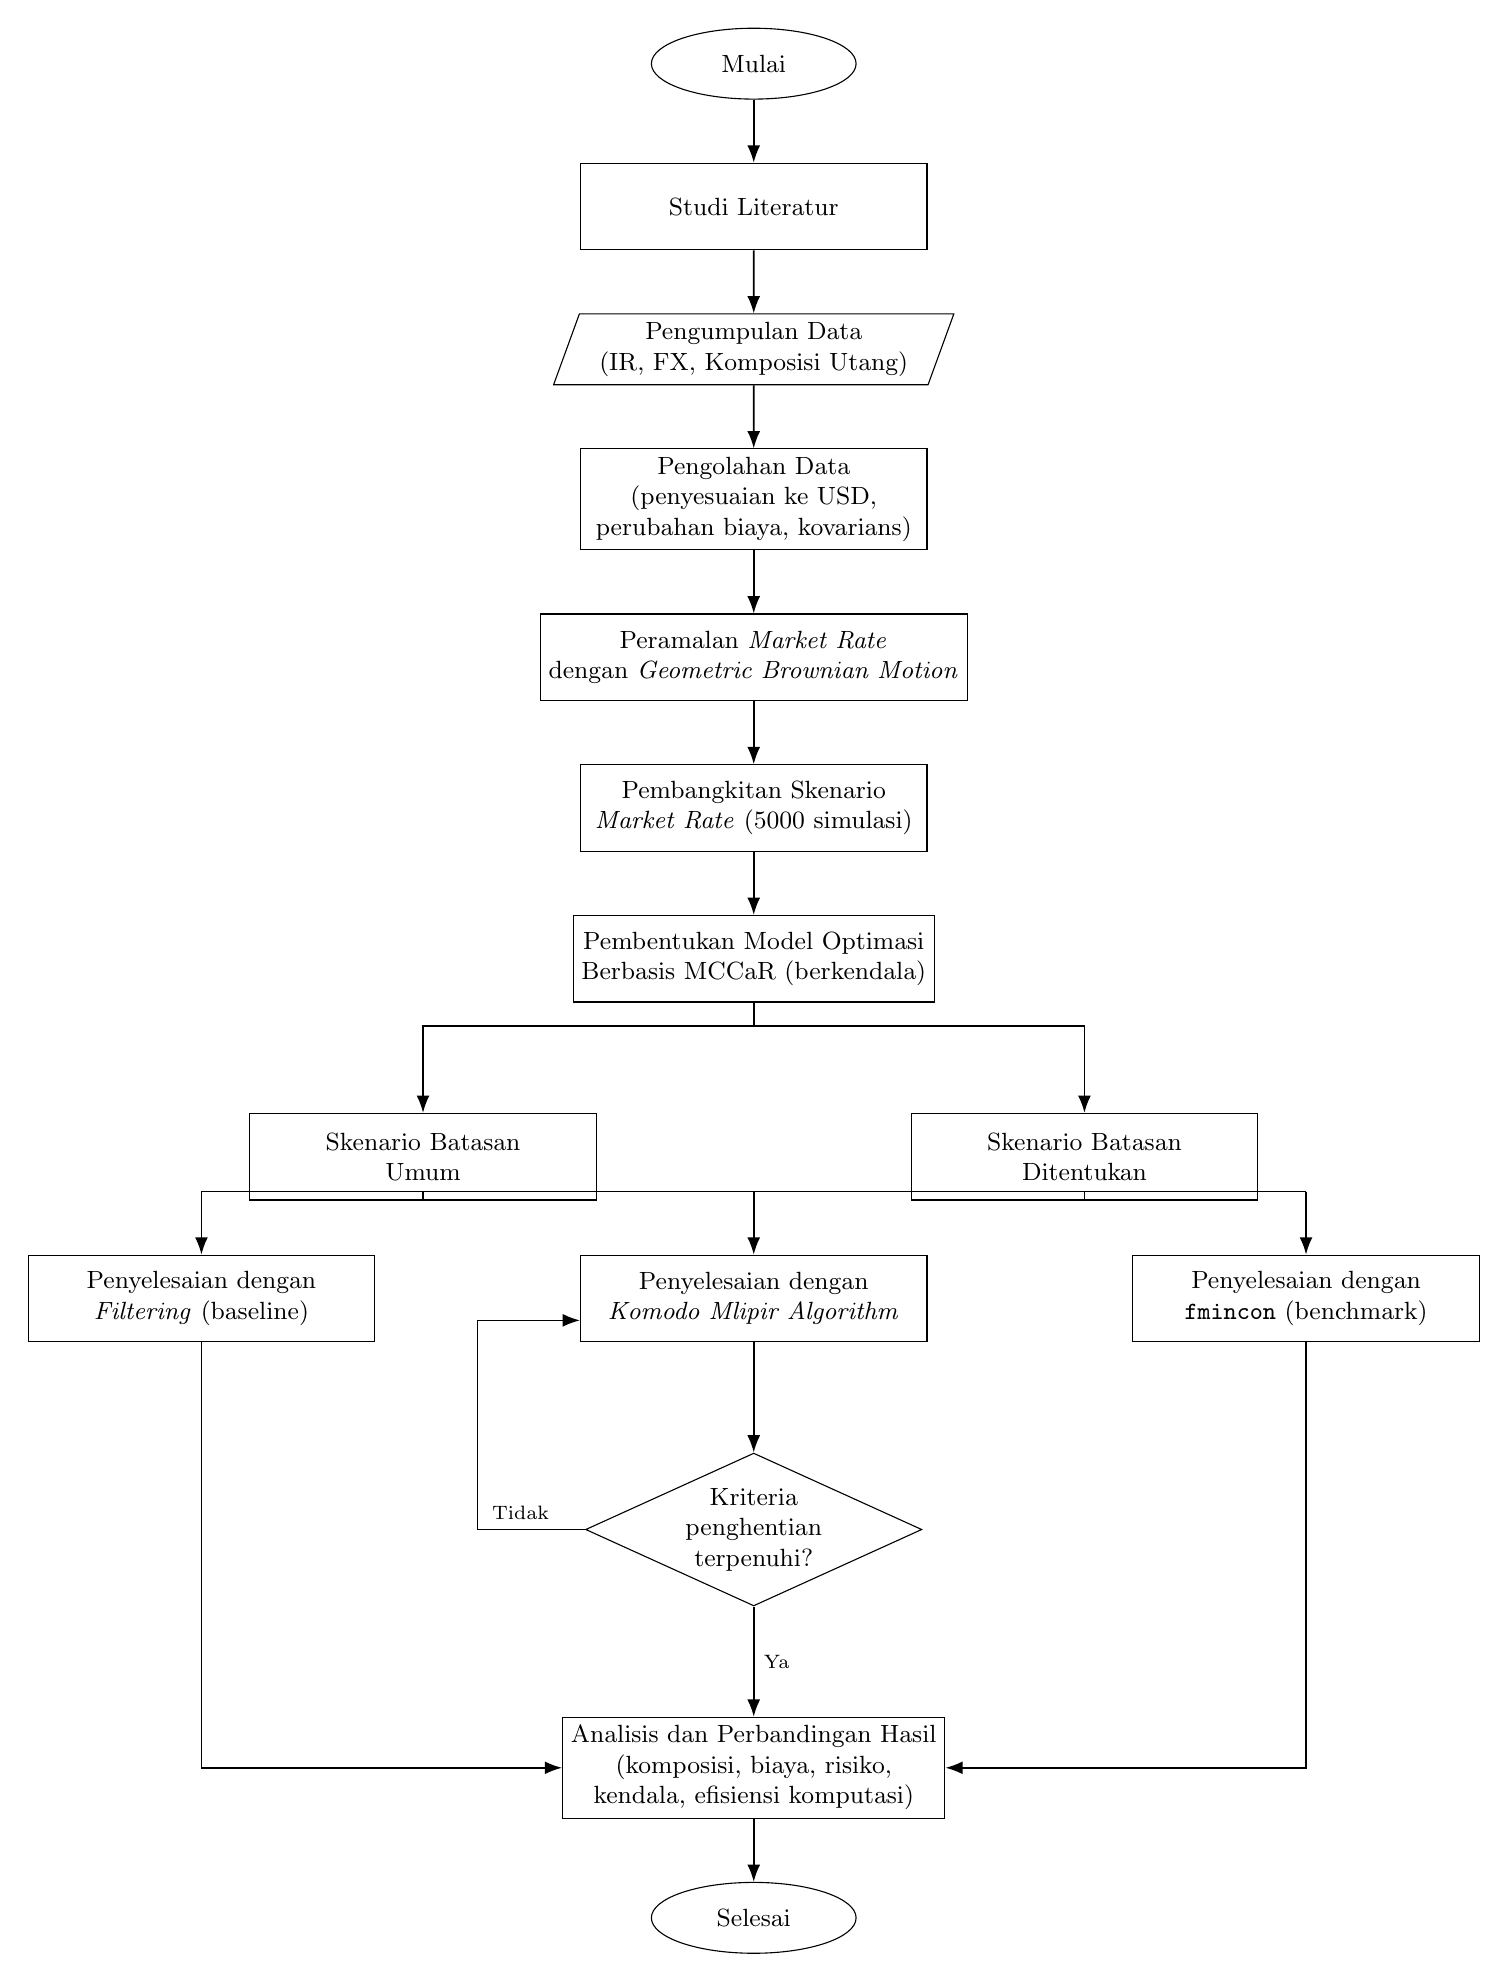
\begin{tikzpicture}[
    node distance = 8mm and 16mm,
    font=\small,
    terminal/.style = {ellipse, draw, minimum width=26mm, minimum height=9mm,
                       align=center, inner sep=2pt},
    io/.style       = {trapezium, draw, trapezium left angle=70,
                       trapezium right angle=110, minimum width=34mm,
                       minimum height=9mm, align=center, inner sep=2pt},
    proc/.style     = {rectangle, draw, minimum width=44mm, minimum height=11mm,
                       align=center, inner sep=3pt},
    decision/.style = {diamond, draw, aspect=2.2, align=center, inner sep=1pt,
                       minimum width=34mm},
    arr/.style      = {-{Latex[length=2.2mm]}, semithick},
    line/.style     = {semithick}
]

% ---- Main spine ----
\node[terminal] (mulai) {Mulai};
\node[proc, below=of mulai] (lit) {Studi Literatur};
\node[io, below=of lit] (input) {Pengumpulan Data\\(IR, FX, Komposisi Utang)};
\node[proc, below=of input] (olah) {Pengolahan Data\\(penyesuaian ke USD,\\perubahan biaya, kovarians)};
\node[proc, below=of olah] (gbm) {Peramalan \textit{Market Rate}\\dengan \textit{Geometric Brownian Motion}};
\node[proc, below=of gbm] (skenario) {Pembangkitan Skenario\\\textit{Market Rate} (5000 simulasi)};
\node[proc, below=of skenario] (model) {Pembentukan Model Optimasi\\Berbasis MCCaR (berkendala)};

% ---- Two scenarios ----
\node[proc, below=14mm of model, xshift=-42mm] (umum)  {Skenario Batasan\\Umum};
\node[proc, below=14mm of model, xshift=42mm]  (tentu) {Skenario Batasan\\Ditentukan};

% ---- Three solvers (placed clearly below the scenario row) ----
\node[proc, below=32mm of model] (kma) {Penyelesaian dengan\\\textit{Komodo Mlipir Algorithm}};
\node[proc, left=of kma, xshift=-10mm]  (filter)  {Penyelesaian dengan\\\textit{Filtering} (baseline)};
\node[proc, right=of kma, xshift=10mm] (fmincon) {Penyelesaian dengan\\\texttt{fmincon} (benchmark)};

% ---- Convergence + analysis + end ----
\node[decision, below=14mm of kma] (konv) {Kriteria\\penghentian\\terpenuhi?};
\node[proc, below=14mm of konv] (analisis) {Analisis dan Perbandingan Hasil\\(komposisi, biaya, risiko,\\kendala, efisiensi komputasi)};
\node[terminal, below=of analisis] (selesai) {Selesai};

% ---- Arrows: spine ----
\draw[arr] (mulai) -- (lit);
\draw[arr] (lit) -- (input);
\draw[arr] (input) -- (olah);
\draw[arr] (olah) -- (gbm);
\draw[arr] (gbm) -- (skenario);
\draw[arr] (skenario) -- (model);

% model -> scenarios
\draw[arr] (model.south) -- ++(0,-3mm) -| (umum.north);
\draw[arr] (model.south) -- ++(0,-3mm) -| (tentu.north);

% scenarios -> solver bus (clean: drop below scenarios, single horizontal bus, then into each solver)
\coordinate (busY) at ($(kma.north)+(0,8mm)$);
\draw[line] (umum.south)  -- (umum.south  |- busY);
\draw[line] (tentu.south) -- (tentu.south |- busY);
\draw[line] (filter.north  |- busY) -- (fmincon.north |- busY);  % horizontal bus spanning all solvers
\draw[arr] (filter.north  |- busY) -- (filter.north);
\draw[arr] (kma.north     |- busY) -- (kma.north);
\draw[arr] (fmincon.north |- busY) -- (fmincon.north);

% KMA -> convergence
\draw[arr] (kma) -- (konv);

% "Tidak" loop: decision west -> up through the clear gap -> into KMA bottom-left
\coordinate (loopX) at ($(filter.east)!0.5!(kma.west)$);
\draw[arr] (konv.west) -- node[above,font=\scriptsize,pos=0.6]{Tidak} (loopX |- konv)
           |- ($(kma.south west)!0.5!(kma.west)$);

% "Ya" -> analysis
\draw[arr] (konv.south) -- node[right,font=\scriptsize]{Ya} (analisis.north);

% filter & fmincon -> analysis (enter left/right edges, not overlapping)
\draw[arr] (filter.south)  |- (analisis.west);
\draw[arr] (fmincon.south) |- (analisis.east);

% analysis -> end
\draw[arr] (analisis) -- (selesai);

\end{tikzpicture}%
}
\caption{Diagram Alir Penelitian}
\label{fig:flowchart-mccar}
\end{figure}


%============================================================

\section{Studi Literatur}\label{sec:studi-literatur}
Studi literatur dilakukan untuk membangun landasan teoritis dan metodologis penelitian. Kajian difokuskan pada teori portofolio modern, model \textit{Mean-Variance Optimization} (MVO), ukuran risiko ekor \textit{Conditional Cost-at-Risk} (CCaR) dan turunannya \textit{Marginal Conditional Cost-at-Risk} (MCCaR), peramalan \textit{market rate} menggunakan \textit{Geometric Brownian Motion} (GBM), serta metode metaheuristik, khususnya \textit{Komodo Mlipir Algorithm} (KMA). Melalui studi literatur ini diperoleh dasar untuk merumuskan model, menentukan fungsi objektif dan kendala, serta menetapkan kriteria pembandingan antara hasil KMA dan metode pembanding.

%============================================================

\section{Pengumpulan Data}\label{sec:pengumpulan-data}
Data yang digunakan dalam penelitian ini bersumber dari Direktorat Jenderal Pengelolaan Pembiayaan dan Risiko (DJPPR) Kementerian Keuangan. Data tersebut meliputi data historis suku bunga (\textit{yield}), data nilai tukar valuta asing, serta data komposisi utang valas eksisting beserta batas proporsi setiap instrumen. Periode pengamatan data historis adalah 1 Januari 2014 sampai dengan 24 November 2025, yang mencakup tiga fase kondisi pasar, yaitu sebelum pandemi Covid-19, saat pandemi, dan setelah pandemi.

Instrumen yang dianalisis terdiri atas tujuh instrumen bersuku bunga tetap dalam tiga mata uang keras, sebagaimana dirinci pada Tabel~\ref{tab:instrumen}. Data suku bunga mencakup \textit{yield} ketujuh instrumen, sedangkan data nilai tukar mencakup kurs USD terhadap EUR dan USD terhadap JPY. Pemilihan kedua pasangan nilai tukar tersebut didasarkan pada asumsi posisi kas USD yang selalu tersedia, sehingga instrumen berdenominasi EUR dan JPY perlu dikonversi ke USD pada saat pembayaran.

\begin{table}[H]
    \centering
    \caption{Instrumen Utang Valas yang Dianalisis}
    \label{tab:instrumen}
    \begin{tabularx}{\textwidth}{c l c c X}
    \hline
    \textbf{No.} & \textbf{Instrumen} & \textbf{Mata Uang} & \textbf{Tenor (tahun)}
    & \textbf{Keterangan} \\
    \hline
    1 & USD\_Fixed\_5Y  & USD & 5  & Instrumen acuan mata uang dasar \\
    2 & USD\_Fixed\_10Y & USD & 10 & Instrumen acuan mata uang dasar \\
    3 & USD\_Fixed\_30Y & USD & 30 & Instrumen acuan mata uang dasar \\
    4 & EUR\_Fixed\_7Y  & EUR & 8  & Dikonversi ke USD via kurs USD/EUR \\
    5 & EUR\_Fixed\_10Y & EUR & 10 & Dikonversi ke USD via kurs USD/EUR \\
    6 & JPY\_Fixed\_5Y  & JPY & 5  & Dikonversi ke USD via kurs USD/JPY \\
    7 & JPY\_Fixed\_10Y & JPY & 10 & Dikonversi ke USD via kurs USD/JPY \\
    \hline
    \end{tabularx}
\end{table}

%============================================================

\section{Pengolahan Data}\label{sec:pengolahan-data}
Tahap pengolahan data bertujuan menyiapkan masukan model optimasi. Tahap awal dilakukan dengan pembersihan data, yang meliputi pemeriksaan nilai hilang (\textit{missing values}), penyeragaman format tanggal, dan penyelarasan indeks tanggal antar seri suku bunga dan nilai tukar agar berdimensi identik. Instrumen berdenominasi EUR dan JPY kemudian disesuaikan ke dalam mata uang USD menggunakan data nilai tukar, sedangkan instrumen USD digunakan langsung sebagai mata uang dasar.

Penyesuaian nilai instrumen untuk satu periode pengamatan dinyatakan sebagai berikut.

\begin{equation}
    \label{eq:penyesuaian-fv}
    FV_i = FX_i\,(1 + IR_i).
\end{equation}

dengan keterangan:
\begin{itemize}
    \item $FV_i$ : nilai instrumen ke-$i$ setelah penyesuaian,
    \item $FX_i$ : nilai tukar instrumen ke-$i$ terhadap USD,
    \item $IR_i$ : tingkat suku bunga (\textit{yield}) instrumen ke-$i$.
\end{itemize}

Setelah seluruh instrumen dinyatakan dalam USD, dihitung perubahan biaya historis menggunakan pendekatan logaritmik pada Persamaan~\ref{eq:perubahan-cost}, lalu vektor biaya ekspektasi $\boldsymbol{\mu}$ pada Persamaan~\ref{eq:rata-cost} dan matriks kovarians $\boldsymbol{\Sigma}$ pada Persamaan~\ref{eq:kovarians}. Vektor $\boldsymbol{\mu}$ dan matriks $\boldsymbol{\Sigma}$ menjadi masukan pada pendekatan berbasis Markowitz, sedangkan untuk pendekatan MCCaR, hasil simulasi \textit{market rate} digunakan sebagai dasar perhitungan risiko ekor.

%============================================================

\section{Peramalan \textit{Market Rate}}\label{sec:peramalan-rate}
Perhitungan risiko ekor pada model MCCaR memerlukan sejumlah besar skenario pergerakan \textit{market rate} di masa mendatang. Penelitian ini membangkitkan skenario tersebut menggunakan model GBM sebagaimana dirumuskan pada Persamaan~\ref{eq:gbm-discrete}. Parameter \textit{drift} $\mu$ dan volatilitas $\sigma$ diestimasi dari data historis suku bunga dan nilai tukar pada periode pengamatan. Sebanyak lima ribu lintasan simulasi dibangkitkan untuk menggambarkan variasi kondisi pasar di masa depan. Khusus untuk instrumen EUR dan JPY, proyeksi suku bunga dikonversi ke dalam USD berdasarkan proyeksi nilai tukar USD/EUR dan USD/JPY agar konsisten dengan asumsi posisi kas USD. Hasil simulasi ini menjadi dasar perhitungan biaya dan risiko ekor pada setiap kombinasi proporsi instrumen.

%============================================================

\section{Pembentukan Model Optimasi Portofolio}\label{sec:pembentukan-model}
Model optimasi komposisi utang valas disusun dengan variabel keputusan berupa vektor bobot portofolio $\mathbf{w} = (w_1, w_2, \ldots, w_n)^{\top}$, dengan setiap $w_i$ menyatakan proporsi alokasi utang pada instrumen ke-$i$. Model dilengkapi dengan kendala anggaran agar total bobot bernilai satu dan kendala batas proporsi setiap instrumen.

Fungsi objektif model adalah meminimumkan biaya portofolio dengan tetap mengendalikan risiko ekor MCCaR. Model optimasi dirumuskan sebagai berikut.

\begin{equation}
    \label{eq:model-mccar}
    \begin{aligned}
    &\min_{\mathbf{w}}
    && \boldsymbol{\mu}^{\top}\mathbf{w} \\
    &\text{terhadap kendala}
    && \mathrm{MCCaR}(\mathbf{w}) \leq \tau, \\
    &&& \sum_{i=1}^{n} w_i = 1, \\
    &&& lb_i \leq w_i \leq ub_i, \quad i = 1, 2, \ldots, n.
    \end{aligned}
\end{equation}

dengan keterangan:
\begin{itemize}
    \item $\boldsymbol{\mu}^{\top}\mathbf{w}$ : biaya ekspektasi portofolio,
    \item $\mathrm{MCCaR}(\mathbf{w})$ : ukuran risiko ekor portofolio sebagaimana dirumuskan pada Persamaan~\ref{eq:mccar},
    \item $\tau$ : batas maksimum risiko ekor yang diperbolehkan,
    \item $lb_i,\,ub_i$ : batas bawah dan batas atas proporsi instrumen ke-$i$.
\end{itemize}

Penelitian ini menggunakan dua skenario batasan proporsi. Skenario pertama menggunakan batasan umum $0 \leq w_i \leq 1$ sebagai pembanding dasar. Skenario kedua menggunakan batasan yang ditentukan berdasarkan komposisi utang eksisting, yaitu $lb_i \leq w_i \leq ub_i$ dengan nilai $lb_i$ dan $ub_i$ pada Tabel~\ref{tab:batas-bobot}. Penggunaan dua skenario ini bertujuan melihat pengaruh batasan proporsi terhadap komposisi portofolio, biaya, dan risiko yang dihasilkan.

\begin{table}[H]
    \centering
    \caption{Komposisi Eksisting dan Batas Proporsi Instrumen}
    \label{tab:batas-bobot}
    \begin{tabularx}{\textwidth}{l c X c c c}
    \hline
    \textbf{Instrumen} & \textbf{Mata Uang} & \textbf{Existing (2024)} &
    \textbf{Min} & \textbf{Max} \\
    \hline
    USD\_Fixed\_5Y  & USD & $45{,}95\%$ & $42{,}50\%$ & $49{,}00\%$ \\
    USD\_Fixed\_10Y & USD & $11{,}36\%$ & $10{,}00\%$ & $12{,}50\%$ \\
    USD\_Fixed\_30Y & USD & $14{,}78\%$ & $13{,}00\%$ & $16{,}50\%$ \\
    EUR\_Fixed\_7Y  & EUR & $14{,}39\%$ & $13{,}00\%$ & $15{,}50\%$ \\
    EUR\_Fixed\_10Y & EUR & $2{,}44\%$  & $1{,}50\%$  & $3{,}00\%$ \\
    JPY\_Fixed\_5Y  & JPY & $6{,}67\%$  & $5{,}00\%$  & $8{,}50\%$ \\
    JPY\_Fixed\_10Y & JPY & $4{,}41\%$  & $3{,}00\%$  & $5{,}50\%$ \\
    \hline
    \textbf{Total}  &     & $100{,}00\%$ & & \\
    \hline
    \end{tabularx}
\end{table}

%============================================================

\section{Penyelesaian Model Optimasi}\label{sec:penyelesaian-model}
Penyelesaian model dilakukan menggunakan tiga pendekatan, yaitu dua metode pembanding dan KMA sebagai metode metaheuristik yang menjadi fokus penelitian. Penggunaan dua metode pembanding bertujuan menempatkan KMA terhadap dua acuan yang berbeda peran, yaitu praktik eksisting dan optimasi deterministik.

%============================================================

    \subsection{Penyaringan Kombinasi (\textit{Filtering})}\label{sub:filtering}

    Metode pembanding pertama adalah penyaringan kombinasi acak sebagaimana digunakan pada kajian DJPPR. Sejumlah besar kombinasi proporsi instrumen dibangkitkan secara acak dalam rentang kelayakan pada Tabel~\ref{tab:batas-bobot}, kemudian setiap kombinasi dievaluasi terhadap biaya dan risiko ekor berdasarkan hasil simulasi \textit{market rate}. Komposisi optimum dipilih berdasarkan keseimbangan rasio efisiensi atau tingkat biaya terendah. Pendekatan ini berperan sebagai \textit{baseline} praktik karena merepresentasikan prosedur yang telah digunakan, namun tidak menjamin diperolehnya solusi optimal.

%============================================================

    \subsection{Optimasi Numerik (\texttt{fmincon})}\label{sub:fmincon}
Metode pembanding kedua adalah optimasi numerik deterministik menggunakan fungsi \texttt{fmincon} pada MATLAB. Fungsi objektif yang diminimumkan adalah biaya
portofolio, sedangkan kendala risiko ekor MCCaR dimasukkan sebagai kendala nonlinear, bersama kendala anggaran dan batasan proporsi. Hasil \texttt{fmincon} digunakan sebagai acuan (\textit{benchmark}) dalam mengevaluasi kualitas solusi
KMA. Karena fungsi berbasis CCaR bersifat tidak mulus, hasil \texttt{fmincon} diinterpretasikan dengan mempertimbangkan keterbatasan metode gradien pada fungsi semacam itu.

%============================================================

    \subsection{\textit{Komodo Mlipir Algorithm} (KMA)}\label{sub:kma-impl}

    Pendekatan ketiga menggunakan KMA. Dalam implementasinya, setiap individu dalam populasi KMA merepresentasikan satu kandidat solusi berupa vektor bobot portofolio. Setiap kandidat solusi dievaluasi berdasarkan fungsi objektif biaya portofolio dan diperiksa terhadap kendala anggaran, batasan proporsi, serta kendala risiko ekor MCCaR. Kandidat solusi yang melanggar kendala diperbaiki melalui penyesuaian bobot atau dikenai penalti pada nilai fungsi objektif agar tidak terpilih sebagai solusi terbaik. Mekanisme pergerakan \textit{big males}, reproduksi \textit{female}, gerakan \textit{small males}, dan adaptasi ukuran populasi mengikuti perumusan pada Subbab~\ref{sec:kma}. Proses iterasi dihentikan berdasarkan kriteria gabungan pada Persamaan~\ref{eq:stopping}.
    
    Penyelesaian dilakukan pada dua skenario batasan proporsi, yaitu batasan umum dan batasan yang ditentukan, sehingga diperoleh hasil optimasi pada kedua
    skenario untuk masing-masing metode.

%============================================================

\section{Analisis Hasil}\label{sec:analisis-hasil}
    
Analisis hasil dilakukan dengan membandingkan solusi yang diperoleh dari KMA terhadap kedua metode pembanding. Aspek yang dianalisis meliputi komposisi proporsi instrumen, nilai biaya portofolio, tingkat risiko ekor MCCaR, pemenuhan kendala, pola konvergensi KMA, dan waktu komputasi. Hasil \texttt{fmincon} digunakan sebagai acuan utama, sedangkan hasil penyaringan kombinasi digunakan sebagai pembanding praktik eksisting. Kedekatan solusi KMA terhadap kedua acuan tersebut menjadi dasar penilaian kelayakan KMA sebagai metode penyelesaian model optimasi komposisi utang valas berbasis MCCaR.

%============================================================

\section{Penarikan Kesimpulan dan Saran}\label{sec:kesimpulan-saran} 
Tahap akhir penelitian adalah penarikan kesimpulan berdasarkan hasil pembentukan model, penyelesaian optimasi, dan analisis perbandingan antara KMA dan metode pembanding. Kesimpulan diarahkan untuk menjawab rumusan masalah penelitian, khususnya mengenai formulasi model optimasi komposisi utang valas berbasis MCCaR serta kemampuan KMA dalam menghasilkan solusi yang mendekati metode pembanding. Selanjutnya, saran disusun untuk memberikan arahan pengembangan penelitian, baik dari sisi perluasan model, penggunaan model peramalan \textit{market rate} yang menangkap sifat \textit{mean reversion}, penambahan kendala yang lebih realistis, maupun pengujian sensitivitas parameter KMA.